\documentclass{beamer}
% \usetheme{Frankfurt}
\usecolortheme{default}
% \usepackage{hyperref}
% \usepackage[utf8]{inputenc} % this is needed for german umlauts
% \usepackage[english]{babel} % this is needed for german umlauts
% \usepackage[T1]{fontenc}    % this is needed for correct output of umlauts in pdf
\usepackage{braket} % for set
\usepackage[nobookmark]{incgraph}
\usepackage{myStyle}

\begin{document}
\selectlanguage{english}

\title{\titleText}
\date{ }
\subject{Machine Learning}

\frame{\titlepage}

\section{ML-KA}
\subsection{ML-KA}
\begin{frame}{Was ist ML-KA?}
    \begin{itemize}
        \item Kurz für \textbf{Machine Learning Karlsruhe}
        \item \textbf{Hochschulgruppe} seit 15.~Oktober 2015
        \item \textbf{Ziel}: Wissen über ML Verbreiten / Mehren
        \item \textbf{Idee}: Forum für interessierte Studenten bilden,
              organisation in kleinen Gruppen
        \item \textbf{Umsetzung} bisher
        \begin{itemize}
            \item Paper Discussion Group (PDG, wöchentlich)
            \item Gesellschaftliche Implikationen vom ML (GIML, 2-wöchentlich)
            \item Teilnahme (und Preisträger) der Herbsttagung der Gesellschaft
                  für Datenanalyse und Numerische Klassifikation
        \end{itemize}
        \item Mehr auf \href{https://ml-ka.de/}{https://ml-ka.de}
    \end{itemize}
\end{frame}

\begin{frame}{Wer ist ML-KA?}
    \begin{itemize}
        \item Vorstand:
        \begin{itemize}
            \item Martin Thoma (info@martin-thoma.de)
            \item Marvin Teichmann
            \item Marvin Schweizer
        \end{itemize}
        \item Mitglieder: Überwiegend aktuelle Studenten des KIT
        \begin{itemize}
            \item 20~Mitglieder (Stand: 3. Februar 2016)
            \item 213 Facebook Mitglieder (Stand: 26. Mai 2016)
        \end{itemize}
    \end{itemize}
\end{frame}

\section{ML}
\subsection{ML}
\begin{frame}{Was ist Machine Learning?}
    \begin{figure}[ht]
        \begin{minipage}[b]{0.45\linewidth}
            \centering
            \includegraphics[width=\textwidth]{../images/traditional-model.png}
            \caption{Traditional Development Model}
        \end{minipage}
        \hspace{0.5cm}
        \begin{minipage}[b]{0.45\linewidth}
            \centering
            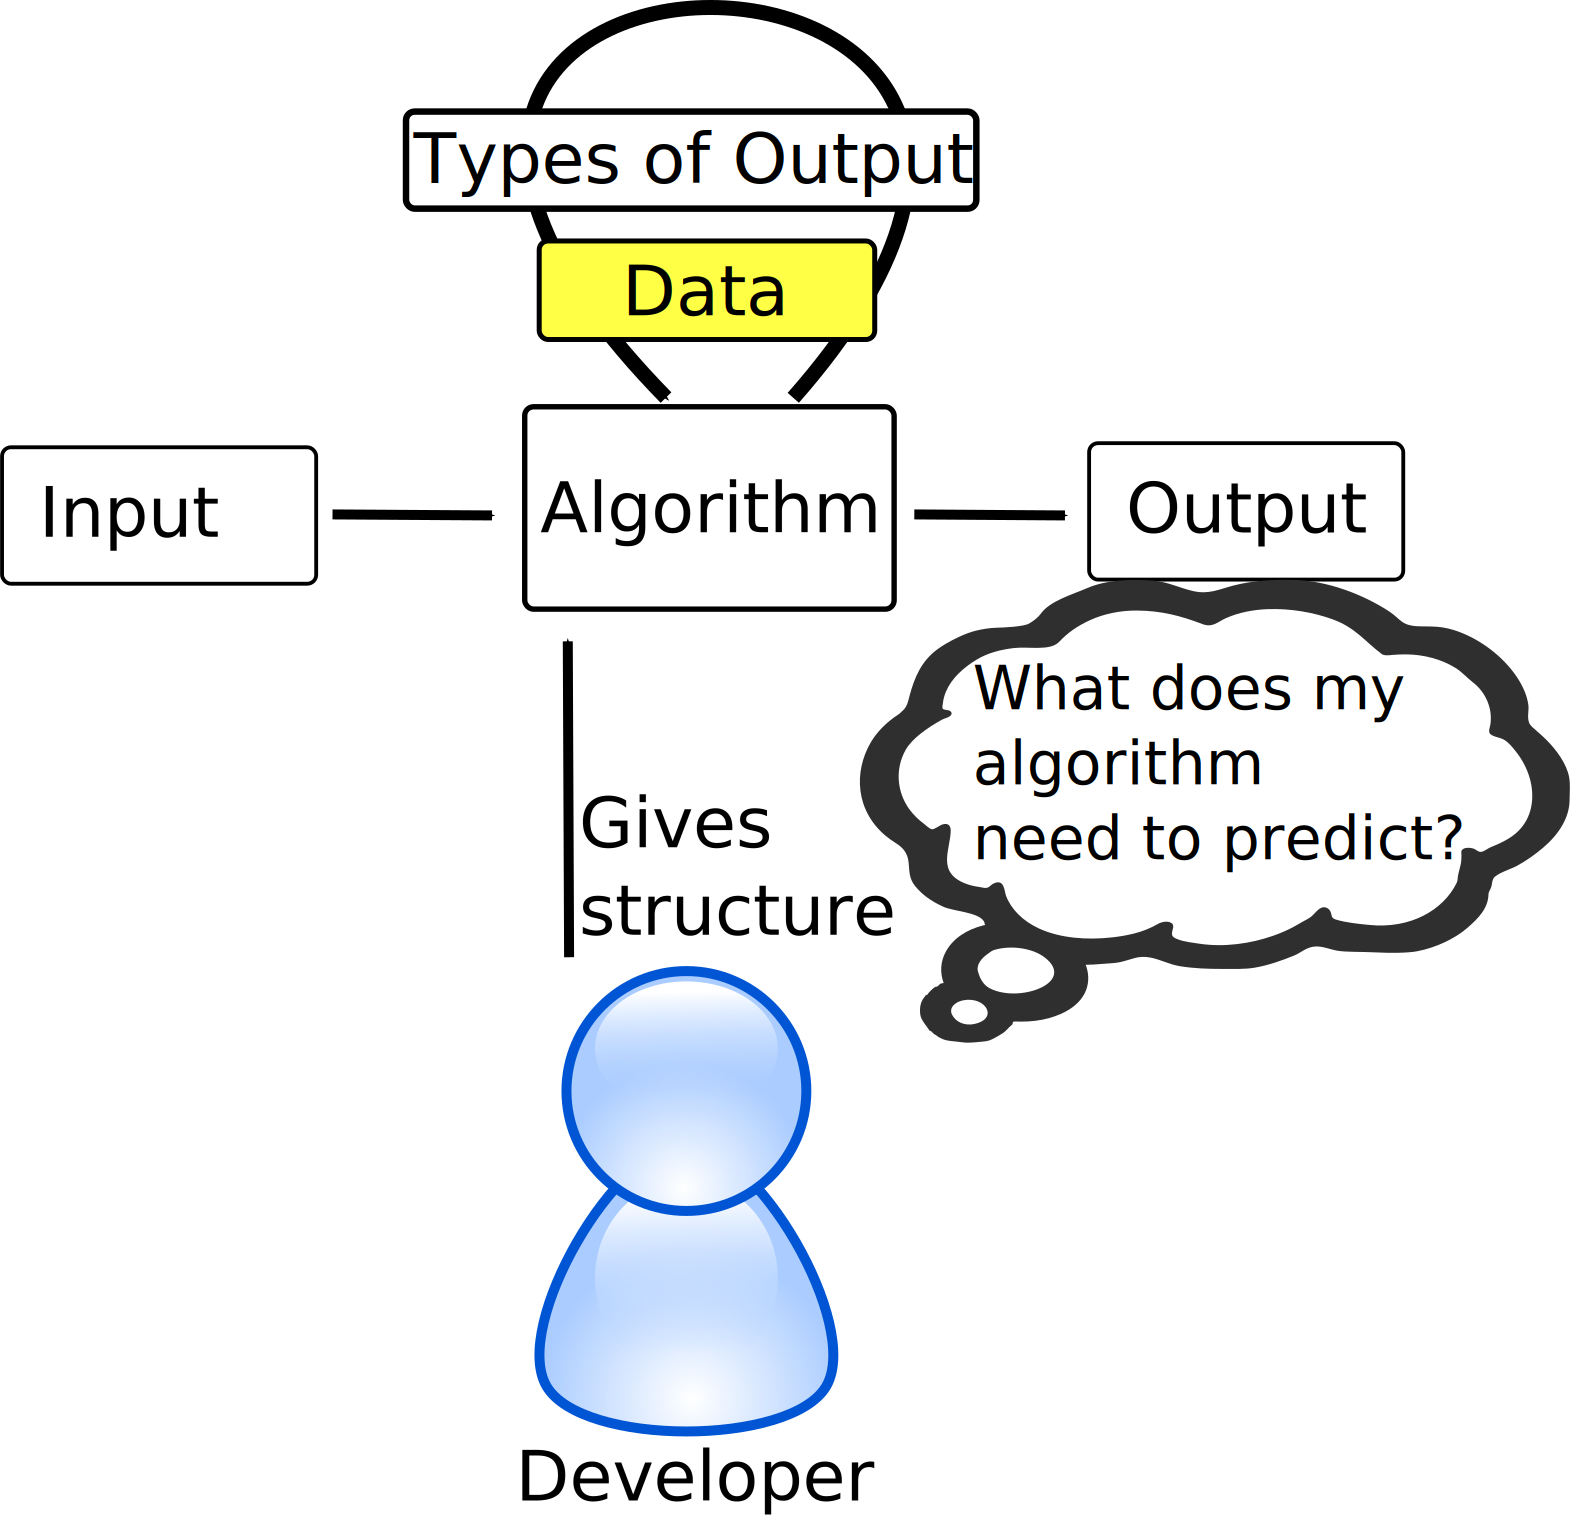
\includegraphics[width=\textwidth]{../images/ml-model.png}
            \caption{ML Model}
        \end{minipage}
    \end{figure}
\end{frame}


\begin{frame}{Problemtypen}
        \begin{minipage}[b]{0.45\linewidth}
            \begin{figure}
            \centering
            \only<1>{\includegraphics[width=\textwidth]{../images/regression-linear-least-squares-2-only-points.png}}
            \only<2->{\includegraphics[width=\textwidth]{../images/regression-linear-least-squares-2.png}}
            \caption{Regression}
            \label{fig:Regression}
            \end{figure}
        \end{minipage}
        \hspace{0.5cm}
        \begin{minipage}[b]{0.45\linewidth}
        \begin{figure}
            \centering
            \only<3>{\vspace*{-0.5cm}\includegraphics[width=\textwidth]{../images/classification-only.png}}
            \only<4>{\includegraphics[width=\textwidth]{../images/clustering-grey.png}}
            \only<5->{\includegraphics[width=\textwidth]{../images/clustering.png}}
            \caption{\only<3>{Klassifikation (überwacht)}\only<4->{und Clustering (unüberwacht)}}
            \label{fig:Klassifikation}
            \end{figure}
        \end{minipage}
\end{frame}


\begin{frame}{Was ist Machine Learning?}
    \begin{figure}
        \centering
        \includegraphics[width=\textwidth, height=0.8\textheight,keepaspectratio]{../images/collaborative-filtering.png}
        \caption{Collaborative Filtering}
    \end{figure}
\end{frame}


\begin{frame}{Was ist Machine Learning?}
    \begin{figure}
        \centering
        \includegraphics[width=\textwidth, height=0.8\textheight,keepaspectratio]{../images/rl.jpg}
        \caption{Reinforcement Learning (RL)}
    \end{figure}
\end{frame}

\section{MNIST}
\subsection{MNIST}
\begin{frame}{MNIST - Ziffern klassifizieren}
    \begin{minipage}[b]{0.45\linewidth}
        \begin{itemize}
            \item Klassen: 0, 1, 2, 3, 4, 5, 6, 7, 8, 9
            \item \num{60000} Trainigsdaten, \num{10000} Testdaten
                  auf \href{http://yann.lecun.com/exdb/mnist/}{yann.lecun.com/exdb/mnist}
            \item Algorithmen zur Klassifizierung: \textbf{SVMs} (Support Vector Machines),
                  \textbf{CNNs} (Convolutional Neural Networks),
                  $k$~Nearest Neighbors (siehe \href{http://martin-thoma.com/k-nearest-neighbor-classification-interactive-example/}{tinyurl.com/knn-interact})
        \end{itemize}
    \end{minipage}
    \hspace{0.5cm}
    \begin{minipage}[b]{0.45\linewidth}
        \begin{figure}
            \centering
            \includegraphics[width=\textwidth]{../images/mnist-2.png}
            \caption{Datensatz der Klasse \enquote{2}; $\SI{28}{\pixel} \times \SI{28}{\pixel}$}
            \label{fig:spline}
        \end{figure}
    \end{minipage}
\end{frame}


\begin{frame}{Wie löst man das?}
    \begin{itemize}[<+->]
        \item \textbf{Situation}: Daten im $\mathbb{R}^{28 \times 28}$,
              Lösungen in $\Set{0, 1, 2, 3, 4, 5, 6, 7, 8, 9}$
        \item ... oder $[0, 1]^{10}$, wenn wir eine Wahrscheinlichkeitsverteilung wollen
        \item \textbf{Lösung}: Neuronale Netze!
    \end{itemize}
\end{frame}

\section{Neuronale Netze}
\subsection{Neuronale Netze}
\incgraph{../images/perceptron-unit.pdf}
\incgraph{../images/feed-forward-perceptron.pdf}

\begin{frame}{}
    \begin{center}
        \Huge Wie finden wir die Gewichte?


        \uncover<2->{Gradientenabstieg (Mehrdimensionale Ableitung)}
    \end{center}
\end{frame}


\begin{frame}{Gradientenabstieg}
    \includegraphics[width=\textwidth, height=0.8\textheight, keepaspectratio]{../images/visualizing-optimization-algos-0.png}

    Quelle: \href{http://imgur.com/a/Hqolp}{http://imgur.com/a/Hqolp}
\end{frame}


\begin{frame}{ImageNet}
    \begin{figure}
        \centering
        \includegraphics[width=\textwidth,height=0.7\textheight,keepaspectratio]{../images/prototypes-thomas-deselaers.jpg}
        \caption{Image by Thomas Deselaers\newline\num{21841}~Synsets, \num{14197122} Bilder}
        \label{fig:image-net}
    \end{figure}
\end{frame}


\section{Tools}
\subsection{sklearn}
\framedgraphic{sklearn}{../images/peekaboo-vision-blogspot-de.png}
\begin{frame}{Weitere Tools}
    \begin{itemize}
        \item TensorFlow (\href{https://www.tensorflow.org/versions/r0.8/tutorials/index.html}{Tutorials})
        \item \href{https://github.com/Russell91/TensorBox}{TensorBox} basiert auf TensorFlow, Lokalisierung (Computer Vision)
        \item \href{http://keras.io/}{Keras}: Sehr einfach zu bedienen,
              abstrahiert von TensorFlow
        \item Datenvisualisierung
            \begin{itemize}
                \item \href{http://pandas.pydata.org/}{Pandas}
                \item \href{https://web.stanford.edu/~mwaskom/software/seaborn/}{Seaborn}
            \end{itemize}
    \end{itemize}
\end{frame}

\end{document}
